\documentclass[10pt,letterpaper]{hmcpset}
\usepackage[margin=1in]{geometry}
\usepackage{graphicx}
\usepackage{amsthm}
\usepackage[shortlabels]{enumitem}
\usepackage{amsmath}
\setlength{\parindent}{0 pt}
\setlength{\parskip}{1 em}
\usepackage{hyperref}
\hypersetup{
colorlinks=true,
linkcolor=blue,
filecolor=magenta,      
urlcolor=cyan,
}

% Theorems
\usepackage{amsthm}
\renewcommand\qedsymbol{$\blacksquare$}
\makeatletter
\@ifclassloaded{article}{
    \newtheorem{definition}{Definition}[section]
    \newtheorem{example}{Example}[section]
    \newtheorem{theorem}{Theorem}[section]
    \newtheorem{corollary}{Corollary}[theorem]
    \newtheorem{lemma}{Lemma}[theorem]
}{
}
\makeatother

% Random Stuff
\setlength\unitlength{1mm}

\newcommand{\insertfig}[3]{
\begin{figure}[htbp]\begin{center}\begin{picture}(120,90)
\put(0,-5){\includegraphics[width=12cm,height=9cm,clip=]{#1}}\end{picture}\end{center}
\caption{#2}\label{#3}\end{figure}}

\newcommand{\insertxfig}[4]{
\begin{figure}[htbp]
\begin{center}
\leavevmode \centerline{\resizebox{#4\textwidth}{!}{\input
#1.pstex_t}}
\caption{#2} \label{#3}
\end{center}
\end{figure}}

\long\def\comment#1{}

\newcommand\abs[1]{\left\lvert#1\right\rvert}
\newcommand\norm[1]{\left\lVert#1\right\rVert}
\DeclareMathOperator*{\argmin}{arg\,min}
\DeclareMathOperator*{\argmax}{arg\,max}

% bb font symbols
\newfont{\bbb}{msbm10 scaled 700}
\newcommand{\CCC}{\mbox{\bbb C}}

\newfont{\bbf}{msbm10 scaled 1100}
\newcommand{\CC}{\mbox{\bbf C}}
\newcommand{\PP}{\mbox{\bbf P}}
\newcommand{\RR}{\mbox{\bbf R}}
\newcommand{\QQ}{\mbox{\bbf Q}}
\newcommand{\ZZ}{\mbox{\bbf Z}}
\renewcommand{\SS}{\mbox{\bbf S}}
\newcommand{\FF}{\mbox{\bbf F}}
\newcommand{\GG}{\mbox{\bbf G}}
\newcommand{\EE}{\mbox{\bbf E}}
\newcommand{\NN}{\mbox{\bbf N}}
\newcommand{\KK}{\mbox{\bbf K}}
\newcommand{\KL}{\mbox{\bbf KL}}

% Vectors
\renewcommand{\aa}{{\bf a}}
\newcommand{\bb}{{\bf b}}
\newcommand{\cc}{{\bf c}}
\newcommand{\dd}{{\bf d}}
\newcommand{\ee}{{\bf e}}
\newcommand{\ff}{{\bf f}}
\renewcommand{\gg}{{\bf g}}
\newcommand{\hh}{{\bf h}}
\newcommand{\ii}{{\bf i}}
\newcommand{\jj}{{\bf j}}
\newcommand{\kk}{{\bf k}}
\renewcommand{\ll}{{\bf l}}
\newcommand{\mm}{{\bf m}}
\newcommand{\nn}{{\bf n}}
\newcommand{\oo}{{\bf o}}
\newcommand{\pp}{{\bf p}}
\newcommand{\qq}{{\bf q}}
\newcommand{\rr}{{\bf r}}
\renewcommand{\ss}{{\bf s}}
\renewcommand{\tt}{{\bf t}}
\newcommand{\uu}{{\bf u}}
\newcommand{\ww}{{\bf w}}
\newcommand{\vv}{{\bf v}}
\newcommand{\xx}{{\bf x}}
\newcommand{\yy}{{\bf y}}
\newcommand{\zz}{{\bf z}}
\newcommand{\0}{{\bf 0}}
\newcommand{\1}{{\bf 1}}

% Matrices
\newcommand{\Ab}{{\bf A}}
\newcommand{\Bb}{{\bf B}}
\newcommand{\Cb}{{\bf C}}
\newcommand{\Db}{{\bf D}}
\newcommand{\Eb}{{\bf E}}
\newcommand{\Fb}{{\bf F}}
\newcommand{\Gb}{{\bf G}}
\newcommand{\Hb}{{\bf H}}
\newcommand{\Ib}{{\bf I}}
\newcommand{\Jb}{{\bf J}}
\newcommand{\Kb}{{\bf K}}
\newcommand{\Lb}{{\bf L}}
\newcommand{\Mb}{{\bf M}}
\newcommand{\Nb}{{\bf N}}
\newcommand{\Ob}{{\bf O}}
\newcommand{\Pb}{{\bf P}}
\newcommand{\Qb}{{\bf Q}}
\newcommand{\Rb}{{\bf R}}
\newcommand{\Sb}{{\bf S}}
\newcommand{\Tb}{{\bf T}}
\newcommand{\Ub}{{\bf U}}
\newcommand{\Wb}{{\bf W}}
\newcommand{\Vb}{{\bf V}}
\newcommand{\Xb}{{\bf X}}
\newcommand{\Yb}{{\bf Y}}
\newcommand{\Zb}{{\bf Z}}

% Calligraphic
\newcommand{\Ac}{{\cal A}}
\newcommand{\Bc}{{\cal B}}
\newcommand{\Cc}{{\cal C}}
\newcommand{\Dc}{{\cal D}}
\newcommand{\Ec}{{\cal E}}
\newcommand{\Fc}{{\cal F}}
\newcommand{\Gc}{{\cal G}}
\newcommand{\Hc}{{\cal H}}
\newcommand{\Ic}{{\cal I}}
\newcommand{\Jc}{{\cal J}}
\newcommand{\Kc}{{\cal K}}
\newcommand{\Lc}{{\cal L}}
\newcommand{\Mc}{{\cal M}}
\newcommand{\Nc}{{\cal N}}
\newcommand{\Oc}{{\cal O}}
\newcommand{\Pc}{{\cal P}}
\newcommand{\Qc}{{\cal Q}}
\newcommand{\Rc}{{\cal R}}
\newcommand{\Sc}{{\cal S}}
\newcommand{\Tc}{{\cal T}}
\newcommand{\Uc}{{\cal U}}
\newcommand{\Wc}{{\cal W}}
\newcommand{\Vc}{{\cal V}}
\newcommand{\Xc}{{\cal X}}
\newcommand{\Yc}{{\cal Y}}
\newcommand{\Zc}{{\cal Z}}

% Bold greek letters
\newcommand{\alphab}{\hbox{\boldmath$\alpha$}}
\newcommand{\betab}{\hbox{\boldmath$\beta$}}
\newcommand{\gammab}{\hbox{\boldmath$\gamma$}}
\newcommand{\deltab}{\hbox{\boldmath$\delta$}}
\newcommand{\etab}{\hbox{\boldmath$\eta$}}
\newcommand{\lambdab}{\hbox{\boldmath$\lambda$}}
\newcommand{\epsilonb}{\hbox{\boldmath$\epsilon$}}
\newcommand{\nub}{\hbox{\boldmath$\nu$}}
\newcommand{\mub}{\hbox{\boldmath$\mu$}}
\newcommand{\zetab}{\hbox{\boldmath$\zeta$}}
\newcommand{\phib}{\hbox{\boldmath$\phi$}}
\newcommand{\psib}{\hbox{\boldmath$\psi$}}
\newcommand{\thetab}{\hbox{\boldmath$\theta$}}
\newcommand{\taub}{\hbox{\boldmath$\tau$}}
\newcommand{\omegab}{\hbox{\boldmath$\omega$}}
\newcommand{\xib}{\hbox{\boldmath$\xi$}}
\newcommand{\sigmab}{\hbox{\boldmath$\sigma$}}
\newcommand{\pib}{\hbox{\boldmath$\pi$}}
\newcommand{\rhob}{\hbox{\boldmath$\rho$}}

\newcommand{\Gammab}{\hbox{\boldmath$\Gamma$}}
\newcommand{\Lambdab}{\hbox{\boldmath$\Lambda$}}
\newcommand{\Deltab}{\hbox{\boldmath$\Delta$}}
\newcommand{\Sigmab}{\hbox{\boldmath$\Sigma$}}
\newcommand{\Phib}{\hbox{\boldmath$\Phi$}}
\newcommand{\Pib}{\hbox{\boldmath$\Pi$}}
\newcommand{\Psib}{\hbox{\boldmath$\Psi$}}
\newcommand{\Thetab}{\hbox{\boldmath$\Theta$}}
\newcommand{\Omegab}{\hbox{\boldmath$\Omega$}}
\newcommand{\Xib}{\hbox{\boldmath$\Xi$}}

% mixed symbols
\newcommand{\sinc}{{\hbox{sinc}}}
\newcommand{\diag}{{\hbox{diag}}}
\renewcommand{\det}{{\hbox{det}}}
\newcommand{\trace}{{\hbox{tr}}}
\newcommand{\tr}{\trace}
\newcommand{\sign}{{\hbox{sign}}}
\renewcommand{\arg}{{\hbox{arg}}}
\newcommand{\var}{{\hbox{var}}}
\newcommand{\cov}{{\hbox{cov}}}
\renewcommand{\Re}{{\rm Re}}
\renewcommand{\Im}{{\rm Im}}
\newcommand{\eqdef}{\stackrel{\Delta}{=}}
\newcommand{\defines}{{\,\,\stackrel{\scriptscriptstyle \bigtriangleup}{=}\,\,}}
\newcommand{\<}{\left\langle}
\renewcommand{\>}{\right\rangle}
\newcommand{\Psf}{{\sf P}}
\newcommand{\T}{\top}
\newcommand{\m}[1]{\begin{bmatrix} #1 \end{bmatrix}}


% info for header block in upper right hand corner
\name{Joseph Gardi, Tim Player}
\class{Differential Geometry}
\assignment{Homework 6}
\duedate{Monday, November 4 2019}

\renewcommand{\labelenumi}{{(\alph{enumi})}}

\begin{document}
\section*{A: Read: } 

\begin{itemize}
\item{Baby Do Carmo, Differential Geometry
    of Curves and Surfaces:  
Sections 2-4, 2-5, 2-6 and Section 5-10 on Abstract surfaces (starting 
on page 425)} 
\item{Handouts 8 and 9}
\item{Lecture Notes}
\end{itemize}

\textbf{B: Problems from Lectures}


\begin{problem}
a) Let $S$ be a subset of $R^3$.  Show that $S$ is a
regular surface if and only if S is locally diffeomorphic 
to $R^2$.
\end{problem}
\begin{solution}
Let $S$ be a regular surface. Then, according to do Carmo, Proposition 2, Chapter 2.2, any point $p \in S$ is the inverse image of a regular value of some function $f \colon U \subset \RR^2 \to S \subset \RR^3$:
\[
S = \{u, v, f(u,v) \}.
\]
Note here relabeling of axes may be necessary, so that the height function $f$ gives the distance from the $xy$-, $yz$-, or $xz$-plane.

Implicit in the term ``regular value", defined in Definition 2 of the same
chapter, is that the function $f$ is differentiable and has an inverse that is
also differentiable. So $f$ is a diffeomorphism between $S$ and $\RR^2$. Thus, at all points $p \in S$, the regular surface $S$ is locally diffeomorphic to $\RR^2$.

Conversely, let the subset $S \subset \RR^3$ be locally diffeomorphic to $\RR^2$. Then, there necessarily exists some differentiable function $F^{-1} \colon S \to U \subset \RR^2$, where both $F$ and $F^{-1}$ are differentiable. This satisfies conditions 1 and 2 ($\mathbf{x}$ is differentiable, $\mathbf{x}$ is a homeomorphism)  of a regular surface. 

The last condition, of regularity, requires more explanation. The differential $dF \colon \RR^2 \to \RR^3$ is indeed one-to-one since, if it were not, then $F^{-1}$ would not be differentiable because the Jacobian determinants would vanish simultaneously. 

Therefore, $S$ being locally diffeomorphic to $\RR^2$ implies that $S$ is a regular surface, completing the ``if and only if" condition.

\end{solution}

\newpage
\begin{problem}
b) Find five examples of regular surfaces such that each of 
them can be represented as a surface of revolution.  Write down
specifically for each example the generating curve, the rotation 
axis, and the parameterization (as a map) for the surface (including
the domain of the map).
\end{problem}
\begin{solution}
For the following examples, consider a closed curve $C$ in the $xz$-plane with the parametrization
\begin{align*}
    x &= f(v),& z &= g(v),& a&< v < b,& f(v) &>0.
\end{align*}
We rotate $C$ about the $z$-axis to generate the surface of revolution
\[
\mathbf{x}(u,v) = (f(v)\cos u, f(v) \sin u, g(v)).
\]
Then, the following give regular surfaces.
\begin{align*}
    f(v) &= \cos(v) + 5,& g(v) &= \sin(v),& 0 &< v <2\pi\\
    f(v) &= \cos(v - 5) + 5,& g(v) &= \sin(v),& 0 &< v <2\pi\\
    f(v) &= \cos(v) + 5,& g(v) &= 2\sin(v),& 0 &< v <2\pi\\
    f(v) &= \cos(2v) + 5,& g(v) &= \sin(2v),& 0 &< v <\pi \\
    f(v) &= \cos(2v) + 5,& g(v) &= \sin(2v),& 2\pi &< v <4\pi
\end{align*}
For all the above, $0 < u < 2\pi$. Note that, in general, the generating curve does not need to be closed.
\end{solution}

\newpage
\textbf{C: Other Problems}

\begin{problem}
a) Problem 10 on page 81, Section 2-3, Baby Do Carmo.

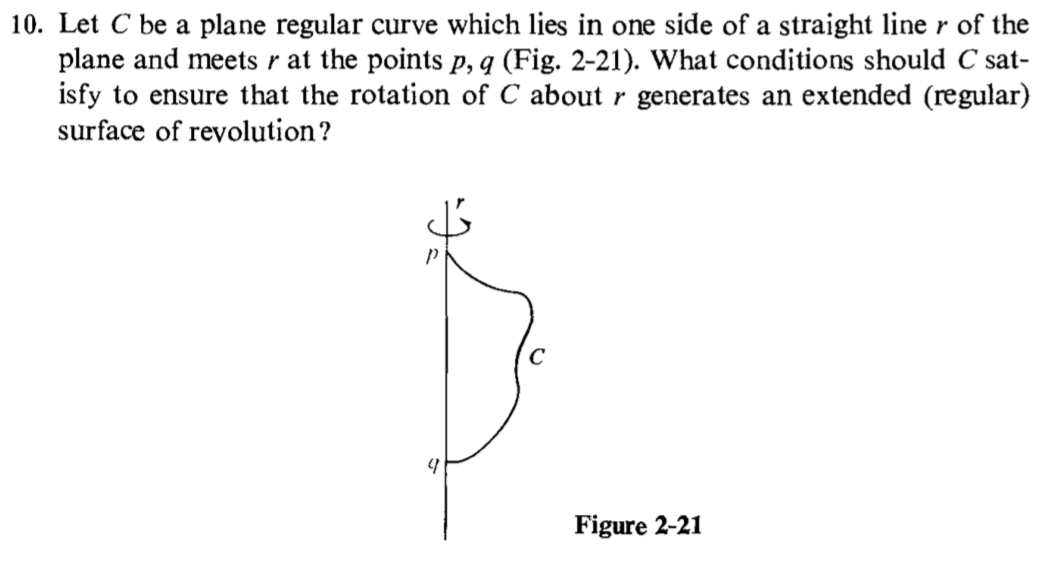
\includegraphics[scale=0.7]{Ca.png}
\end{problem}
\begin{solution}
To result in a regular surface, the $C$ should be perpendicular to $r$ at $p$ and $q$ (otherwise an irregular pinch point would occur). Furthermore, $C$ should be non-self-intersecting.
\end{solution}

\newpage
\begin{problem}
 b) Problem 9 on page 89, Section 2-4, Baby Do Carmo.
 
 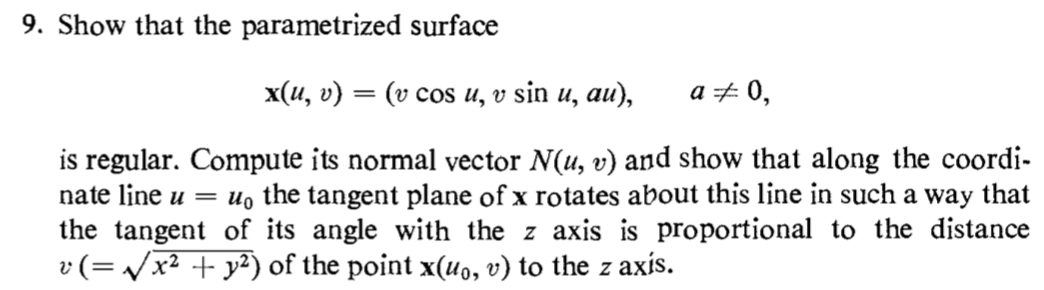
\includegraphics[scale=0.7]{Cb.png}
\end{problem}
\begin{solution}
To be regular, $\mathbf{x}$ must be differentiable, $\mathbf{x}$ must be a homeomorphism, and $d\mathbf{x}_q$ must be one-to-one for each $q \in U$. This is the case.

\textbf{Differentiable}
Clearly, $\mathbf{x}$ is differentiable.

\textbf{Homeomorphism}
$\mathbf{x}$ is a continuous function, and the inverse
\[
u(x,y,z) = z/a, \qquad v(x,y,z) = \sqrt{x^2 + y^2}
\]
is also continuous. Note that we may define other functions for $u$.

\textbf{Regularity}
For each point $q = (u,v) \in \RR^2$, the differential \[
d\mathbf{x}_q = 
\begin{pmatrix}
-v \sin u &\cos u\\
v \cos u & \sin u\\
a &0
\end{pmatrix}
\]
is one-to-one because the Jacobian determinants never vanish simultaneously.
\begin{align*}
    \frac{\partial(x,y)}{\partial(u,v)} &= -v \tag{Vanishes iff $v=0$.}\\
    \frac{\partial(x,z)}{\partial(u,v)} &= -a \cos u
    \tag{Vanishes iff $u = 2\pi n + \pi$.}\\
    \frac{\partial(y,z)}{\partial(u,v)} &= -a \sin u
    \tag{Vanishes iff $u = 2\pi n$.}
\end{align*}
Clearly, the latter two can never vanish simultaneously.
Therefore, the parametrized surface is regular.

\textbf{Normal Vector}
First, an exercise in imagination. Close your eyes. (Okay,  first finish reading this. Then close your eyes.) 

Imagine you are walking up a spiral staircase with a thin rod around the middle. The staircase, of course, is the given helicoid and the thin rod is the $z$-axis. Now, step inward toward the thin rod. You might stumble. Why? Because the length of each step shrinks as you progress radially inward, yet the rise associated with each step remains the same. The closer in you get, the steeper the steps seem to become. Let's formalize that.

Define the normal vector $N(u,v) = x_u \wedge x_v$. Then,
\begin{align*}
    N(u,v) &= 
\begin{vmatrix}
i &j &k\\
-v\sin u & v\cos u & a\\
\cos u & \sin u & 0
\end{vmatrix} =
\begin{pmatrix}
a \sin u\\
a \cos u\\
-v
\end{pmatrix}.
\end{align*}
This vector tells us the tangent of the angle $\theta$ between the normal vector and the $z$-axis (AKA, the steepness of the spiral staircase). Reading directly off the coordinates, we can see that the projection of $N$ onto the $z$-axis is $-v$, while the component orthogonal to the $z$-axis has magnitude $a$. Therefore, $\tan(\theta) = \frac{a}{v}$. 

Substituting $\alpha = 90 - \theta$ gives the angle of the helicoid surface (not its normal) relative to the $z$-axis and yields the desired proportional relationship.
\end{solution}
\newpage
\begin{problem}
c) Problem 15 on page 90, Section 2-4, Baby Do Carmo.

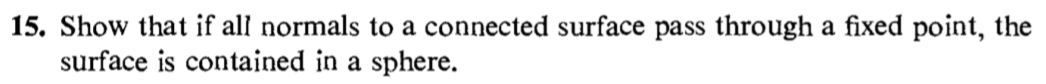
\includegraphics[scale=0.7]{Cc.png}
\end{problem}
\begin{solution}
Suppose that two points $p$ and $q$ on the surface $S$, connected by a curve $\alpha \colon t \in (0, \epsilon) \to S$, have normals passing through a fixed point $c$. 

Then, we claim that $p$ and $q$ must both be the same distance from $c$.

To prove this, suppose that $p$ and $q$ were not the same distance from $c$. Then, along the curve $\alpha$, the distance from $d$ would change. Let $r(x)$ be the distance of a point $x$ from $d$. By the mean value theorem, there exists some value $t \in (0, \epsilon)$ such that $\frac{dr}{dt} \neq 0$.

Yet if, at some point $t$, $\frac{dr}{dt} \neq 0$, this implies that the normal would not pass through $c$, a contradiction. Therefore, $p$ and $q$ must have the same distance from $c$, and furthermore all points along $\alpha$ must be the same distance from $c$.

The above conclusion implies that any two points on the surface are connected by a circular arc. Therefore, the surface is a sphere.
\insertfig{notsphere.jpg}{A picture of points $p$, $q$, and $\alpha(t)$. Note, visually, how the existence of nonzero $dr/dt$ induces a skew in the normal line as the tangent $\alpha'(t)$ contains a component in the $\hat{r}$ direction, making it impossible for the surface to be normal to $c$ there.}{fig:notsphere}
\end{solution}

\newpage
\begin{problem}
d) Problem 18 on page 90, Section 2-4, Baby Do Carmo.

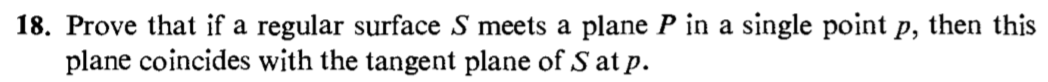
\includegraphics[scale=0.7]{Cd.png}
\end{problem}
\begin{solution}

Let $\psi \colon U \subset \RR^2 \to V \subset P$ be a parametrization for $P$ in a small neighborhood around $p$. That such a function exists is a property of regular surfaces. Let $\psi^{-1}(p) = q = (u_0, v_0)$.

Plainly, $\psi(q) = p \in S \cap P$. That is, the mapping $\psi$ takes $q$ to the plane $P$ as well as the surface $S$.

To prove the desired claim, we will show that the differential $d\psi_p$, whose columns lie within the tangent plane of $S$ at $p$, describes the plane $P$. We will prove this by contradiction.

Suppose that the columns of $d\psi_p = [\psi_u,\psi_v]$ did not lie within $P$. Then, the unit normal vector of $S$,
\[
N(u_0,v_0) = \frac{\psi_u \wedge \psi_v}{\abs{\psi_u \wedge \psi_v}},
\]
would differ from the normal vector to the plane $p$. This would require that $P$ intersect $S$ at more than a single point, as the intersection of two non-parallel planes is a line. (Locally, $S$ behaves as the plane $T_p$. It is unavoidable that $T_p$ being nonparallel to $P$ would result in a local multi-point intersection of $S$ and $P$.)

Thus, $N(u_0, v_0)$ cannot be different from the unit normal of plane $P$; it must be the same. Since $P$ has the same normal vector as $S$ at $p$, and $p \in U \cap S$, $P$ coincides with the tangent plane of $S$ at $p$.

A better proof is given by Professor Lee at

\href{https://math.stackexchange.com/questions/892278/if-a-plane-intersects-a-regular-surface-at-exactly-one-point-then-it-is-the-tan?newreg=1b0c86190e854719923f1b920b3125ea}{https://math.stackexchange.com/questions/892278/if-a-plane-intersects-a-regular-surface-at-exactly-one-point-then-it-is-the-tan?newreg=1b0c86190e854719923f1b920b3125ea}. 

However, the proof I provided is my own. I'm curious about whether my justification in the parentheses is adequate.

\end{solution}

\newpage
\begin{problem}
e) Problem 1 on page 99, Section 2-5, Baby Do Carmo.

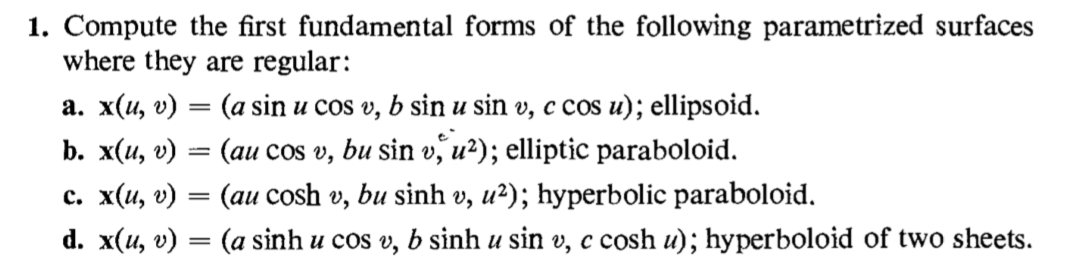
\includegraphics[scale=0.7]{Ce.png}
\end{problem}
\begin{solution}
We will find the $\textbf{x}_u, \textbf{x}_v$ for each problem. From there we
find $E=<\textbf{x}_u, \textbf{x}_u>, F - <\textbf{x}_u, \textbf{x}_v>,
G=<\textbf{u}_v, \textbf{u}_v>$. Then the first fundamental form is,
\begin{align*}
  I_p((u', v')) = E (u')^2 + 2Fu'v' + G(v')^2
\end{align*}
where $p$ is a point on the surface. \\
\begin{enumerate}[(a)]
\item $\textbf{x}_u = (a \cos u \cos v, b \cos u \sin v, -c \sin u),
  \textbf{x}_v = (-a \sin u \sin v, \sin u \cos v, 0)$.
\item $\textbf{x}_u = (a \cos v, b \sin v, 2u), \textbf{x}_v = (-au \sin v, bu
  \cos v, 0)$
\end{enumerate}
\end{solution}

\newpage
\begin{problem}
f) Problem 3 on page 99, Section 2-5, Baby Do Carmo.

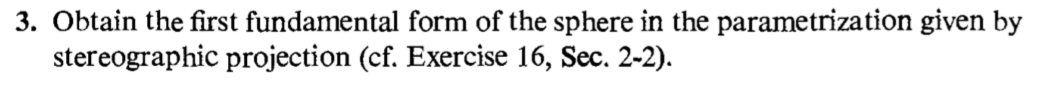
\includegraphics[scale=0.7]{Cf.png}
\end{problem}
The parameterization for the surface is,
\begin{align*}
  \pi^{-1}(u, v) = \begin{bmatrix}
    \frac{4u}{u^2 + v^2 + 4} \\
    \frac{4v}{u^2 + v^2 + 4} \\
    \frac{2(u^2 + v^2)}{u^2 + v^2 + 4}
    \end{bmatrix}
\end{align*}
Then,
\begin{align*}
  \boldsymbol{\pi^{-1}}_u = \begin{bmatrix}
    \frac{4}{u^2 + v^2 + 4} - \frac{4u}{(u^2 + v^2 + 4)^2} \cdot 2u \\
    -\frac{4v}{(u^2 + v^2 + 4)^2} \cdot 2u \\
    \frac{4u}{u^2 + v^2 + 4} - \frac{2(u^2 + v^2)}{(u^2 + v^2 + 4)^2} \cdot 2u
  \end{bmatrix} \\
  \boldsymbol{\pi^{-1}}_v = \begin{bmatrix}
    -\frac{4u}{(u^2 + v^2 + 4)^2} \cdot 2v \\
    \frac{4}{u^2 + v^2 + 4} - \frac{4v}{(u^2 + v^2 + 4)^2} \cdot 2v \\
    \frac{4v}{u^2 + v^2 + 4} - \frac{2(u^2 + v^2)}{(u^2 + v^2 + 4)^2} \cdot 2v
  \end{bmatrix}
\end{align*}
Then calcualate the first fundamental form as described in the last problem. 
\newpage
\begin{problem}
g) Problem 9 on page 100, Section 2-5, Baby Do Carmo.

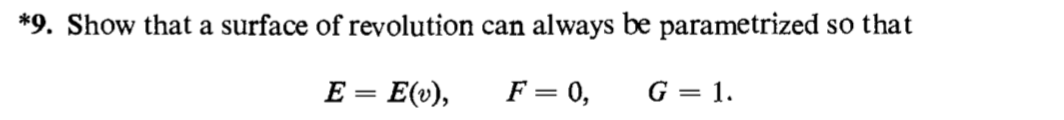
\includegraphics[scale=0.7]{Cg.png}
\end{problem}
%Consider a function $f: R \rightarrow R$ that we want to revolve around the x axis in
%order to obtain a surface of revolution. Then the parameterization for the
%surface would be,
%\begin{align*}
%  \mathbf{x}(u, v) = (f(u) \cos \frac{v}{f(u)}, f(u) \sin \frac{v}{f(u)}, u) 
%\end{align*}
%
%So,
%\begin{align*}
%  \textbf{x}_u = \begin{bmatrix}
%
%    f'(u) \cos \frac{v}{f(u)} - \sin (\frac{v}{f(u)}) \frac{v}{f(u)}f'(u) \\
%    1
%   \end{bmatrix}
%\end{align*}
%for $u \in [0, z_f], v \in [0, 2\pi]$. Then $E=<\textbf{x}_u, \textbf{x}_u> = E(u) $
\newpage
\textbf{D: Extra Credit Problems}

\begin{problem}
a) Let $T\subset R^3$ be a torus of revolution with center in 
$(0,0,0)\in R^3$ and let $A(x,y,z)=(-x,-y,-z)$.
Let $K$ be the quotient space of the torus $T$ by the equivalence 
relation $p\sim A(p)$.  Can you tell what surface $K$ is? 
\end{problem}

\newpage
\begin{problem}
b) Show that $K$ is a differentiable 2-dimensional manifold.
\end{problem}

\newpage
\begin{problem}
c) Show that $K$ is non orientable in two different ways.
\end{problem}

\end{document}

